% Filename  : samplepaper.tex
% Purpose   : A sample exam paper to demonstrate how to use the 'ditpaper'
%             TeX class.
% Author    : Emmet Caulfield
% Revision  : $Id: samplepaper.tex 2 2006-02-19 20:34:45Z emmet $
% Repository: $HeadURL: http://svn.netrogen.lan/tex-ditpaper/trunk/samplepaper.tex $
%

% 'nosolution' (default) and 'solution' toggle the inclusion of solutions
% in the output. The tag --SOLUTION-OPTION--, below, is replaced by 'sed' 
% in the Makefile to cause both the paper and the solutions to be produced.
\documentclass[--SOLUTION-OPTION--]{ditpaper}

\usepackage{rotating}
\usepackage{graphicx}

% These must be set or bizarre defaults will be used:
\facility{Kevin Street, Dublin 8}
\course{BSc (Hons) in Computer Science}
\examcode{S228/406}
\stage{Stage 4}
\session{Semester 2 Examinations 2011}
\title{Artificial Intelligence II}
\examiners{Dr. John Kelleher\\
Dr. D. Lillis\\
Dr. I. Arana}
\examdate{Friday $20^{th}$ May\\4:00 p.m. to 6:00 p.m.\\}
\examtime{\centerline{Duration: 2 Hours}}
\instructions{Answer Question 1 (40 marks) \textbf{and}\par{} any 2 Other Questions (30 marks each).}

\begin{document}


%aima chapters 18
% inductive bias, learning theory - supervised/unsupervised, overfitting, lazy/eager learner, classification v regression, false positive v false negatives, linear separability, consistency, evaluation

\question
\begin{enumerate}
	\item Explain what is meant by \textbf{inductive learning}.
	\marks{5}
	\begin{answer}
		Inductive Learning involves the process of learning by example � where a system tries to induce a general rule from a set of observed instances
	\end{answer}
	\item In the context of machine learning, distinguish between \textbf{supervised} and \textbf{unsupervised} learning.
	\marks{5}
	\begin{answer}
		The distinction is that with \textbf{supervised learning} we know the actual label or category for each piece of data on which we train, whereas with \textbf{unsupervised learning} we do not know the classification of the data in the training sample. Unsupervised learning can thus often be viewed as a \textbf{clustering} task, while supervised learning can usually be seen as a \textbf{classification} task, or equivalently as a function-fitting task where one extrapolates the shape of a function based on some data points.
	\end{answer}	
	\item  Inductive machine learning is often referred to as an \textbf{ill-posed problem}. What is meant by this description?
	\marks{10}
	\begin{answer}
		Inductive machine learning algorithms essentially search through a hypothesis space to find a the best hypothesis that is consistent with the training data used. It is possible to find multiple hypotheses that are  consistent with a given training set (i.e. agrees with all training examples).  It is for this reason that inductive machine learning is referred to as an ill-posed problem as there is typically not enough information in the training data used to build a model to choose a single best hypothesis. Inductive machine learning algorithms must somehow choose one of the available hypotheses as the \emph{best}. An example like that shown in the figure below would be useful at this point
		\begin{center}
			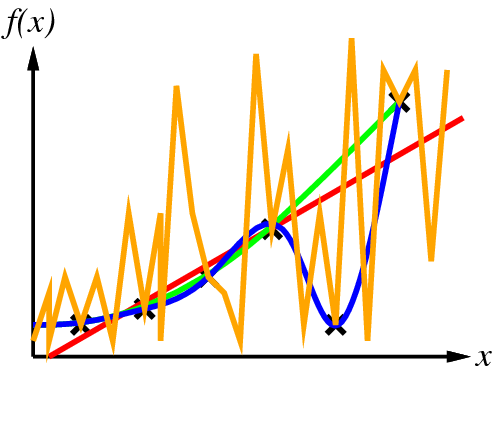
\includegraphics[width=5cm]{./images/curve-fitting5.png}
		\end{center}
	\end{answer}
	\item Let us say we have three classification algorithms. How can we order these three from best to worst?
	\marks{20}
	\begin{answer}
		This is a discursive question so giving a precise answer is not appropriate. However, key points that the student should touch on include:
		\begin{itemize}
		\item Predictive accuracy
		\item Speed and scalability 
		\begin{itemize}
			\item Time to construct the model
			\item Time to use the model
		\end{itemize}
		\item Robustness (handling noise and missing values)
		\item Scalability
		\item Interpretability (understanding and insight provided by the model)
	\end{itemize}
	It should be noted also, that these evaluation criteria are application dependent.
	\end{answer}
\end{enumerate}


\newpage

%Q2
% knn and CBR 
% information theory, entropy, Decision Trees, Inductive logic programming
\begin{table}[htdp]
\caption{Example feature vectors for animal classification. A 1 indicates the animal possesses the feature listed in the column, and 0 indicates they do not. The rightmost column lists the classification of each ainmal.}
\begin{center}
\begin{tabular}{|c|c|c|c|c|c|c|c|c|c|c|}
\hline
Species & \begin{sideways}Births Live Young\end{sideways} & \begin{sideways}Lays Eggs\end{sideways} & \begin{sideways}Feeds Offspring Own Milk\end{sideways} & \begin{sideways}Warm-Blooded\end{sideways}  & \begin{sideways}Cold-Blooded \end{sideways} & \begin{sideways}Land and Water Based\end{sideways} & \begin{sideways}Has Hair \end{sideways} & \begin{sideways}Has Feathers\end{sideways} & Class \\
\hline 
Cat & 1 & 0 & 1 & 1 & 0 & 0 & 1 & 0 & Mammal \\
Frog & 0 & 1 & 0 & 0 & 1 & 1 & 0 & 0 & Amphibian \\
Squirrel & 1 & 0 & 1 & 1 & 0 & 0 & 1 & 0 & Mammal \\
Duck & 0 & 1 & 0 & 1 & 0 & 1 & 0 & 1 & Bird \\
\hline
\end{tabular}
\end{center}
\label{tab:ainmals-classification}
\end{table}%

\begin{table}[htdp]
\caption{The attributes of a newly discovered animal. A 1 indicates the animal possesses the feature listed in the column, and 0 indicates they do not. The column on the right contains a ? because the animal has not yet been classified.}
\begin{center}
\begin{tabular}{|c|c|c|c|c|c|c|c|c|c|c|}
\hline
Species & \begin{sideways}Births Live Young\end{sideways} & \begin{sideways}Lays Eggs\end{sideways} & \begin{sideways}Feeds Offspring Own Milk\end{sideways} & \begin{sideways}Warm-Blooded\end{sideways}  & \begin{sideways}Cold-Blooded \end{sideways} & \begin{sideways}Land and Water Based\end{sideways} & \begin{sideways}Has Hair \end{sideways} & \begin{sideways}Has Feathers\end{sideways} & Class \\
\hline 
Mystery & 0 & 1 & 0 & 0 & 0 & 1 & 0 & 0 & ? \\
\hline
\end{tabular}
\end{center}
\label{tab:animal-attributes}
\end{table}%
		
			
\question 
	\begin{enumerate}
		\item You are working as an assistant-biologist to the Charles Darwin on the Beagle voyage. You are at the Gal\'apagos Islands and you have just discovered a new animal that has not yet been classified. Table \ref{tab:animal-attributes} lists the attributes of the animal you have found. Mr. Darwin has asked you to classify the animal using a nearest-neighbour approach and he has supplied you with a case-base of already classified animals, see Table \ref{tab:ainmals-classification}. 
		\begin{enumerate}
			\item A good measure of distance between two instances with categorical features is the number of features which have different values (the \textbf{overlap metric}, also known as the \textbf{hamming distance}). Using this measure of distance compute the distances between the mystery animal and each of the animals in the case base. 
		\marks{5}
		\begin{answer}
				\begin{center}
					\begin{tabular}{|c|c|c|}
						\hline
						Species & Class & Distance\\
						\hline 
						Cat & Mammal & 6\\
						Frog & Amphibian & 1\\
						Squirrel & Mammal & 6\\
						Duck & Bird & 2\\
						\hline
					\end{tabular}
				\end{center}
		\end{answer}
			\item If you used \textit{1-NN} classification what class would be assigned to the mystery animal?
		\marks{5}
		\begin{answer}
			The nearest neighbor to the mystery animal is the Frog. So the mystery animal would be classified as an amphibian.
		\end{answer}
			\item If the you used \textit{4-NN} classification what class would be assigned to the mystery animal? 
		\marks{5}
		\begin{answer}
				If you applied a $4-NN$ classification to this case-base you would include all the instances in the case-base irrespective of their distance from the test instance feature vector. As a result the test instance would be assigned the most frequently occurring class in the case-base. This would result in the mystery animal being classified as a mammal. 
		\end{answer}
		\end{enumerate}
		% Information theory and Decision Trees
		\item Table \ref{tab:x-y-classification-data} provides a classification for a data set of X Y pairs.		\begin{enumerate}
			\item Calculate the \textbf{entropy} for this classification.
			\marks{5}
			\begin{answer}
				Entropy is $-\frac{3}{5}log_2\frac{3}{5}-\frac{2}{5}log_2\frac{2}{5}=0.971$
			\end{answer}
			\item Calculate the \textbf{information gain} for X and Y.
			\marks{5}
			\begin{answer}
				Entropy for X = T $-\frac{3}{4}log_2\frac{3}{4}-\frac{1}{4}log_2\frac{1}{4}=0.811$\\
				Entropy for X = F $0-\frac{1}{1}log_2\frac{1}{1}=0$\\
				Gain for X $0.971-(\frac{4}{5}\times0.811+\frac{1}{5}\times0)=0.322$\\
				Entropy for Y = T $-\frac{2}{3}log_2\frac{2}{3}-\frac{1}{3}log_2\frac{1}{3}=0.918$\\
				Entropy for Y = F $-\frac{1}{2}log_2\frac{1}{2}-\frac{1}{2}log_2\frac{1}{2}=1.0$\\
				Gain for Y $0.971-(\frac{3}{5}\times0.918+\frac{2}{5}\times1)=0.02$\\
			\end{answer}
		\end{enumerate}
				\begin{table}[h]
			\begin{center}
			\begin{tabular}{|c|c|c|}
				$X$ & $Y$ & Class \\
				\hline
				T & T & + \\
				T & F & - \\
				T & F & + \\
				T & T & + \\
				F & T & - \\
			\end{tabular}
			\end{center}
			\caption{X and Y Classification Data}
			\label{tab:x-y-classification-data}
		\end{table}
		%inductive logic programming
		\item The following sets express the mappings between predicates $r$, $p$, $q$, $s$, $class1$ and $class2$: 
				\begin{itemize}
					\item $r\rightarrow \{a1, a2, a5, a6 \}$, 
					\item $p\rightarrow \{a2, a3, a5, a7 \}$, 
					\item $q\rightarrow \{a1, a2, a6 \}$, 
					\item $s\rightarrow \{(a2, f), (a1,1), (a6,f)\}$, 
					\item $class1\rightarrow \{a2\}$, 
					\item $class2\rightarrow \{a2, a6\}$. 
				\end{itemize}
				Given these sets, give a specialisation of the rule $class1(X)\leftarrow r(X) \land p(X)$ such that the rule is only satisfied by $class1$ members.
		\marks{5}
		\begin{answer}
			$class1(X)\leftarrow r(X) \land p(X) \land q(X)$
		\end{answer}
	\end{enumerate}



\newpage
	
%Q3 30 marks
% basic probability 5
% bayesian networks 10
% bayesian learning  15
\begin{table}[tb]
\caption{Joint Distribution for X and Y}
\begin{center}
\begin{tabular}{c|cc}
                  & $X=x_{1}$ & $X=x_{2}$ \\
                  \hline
$Y=y_{1}$ & 0.02        & 0.30 \\
$Y=y_{2}$ & 0.14        & 0.32\\
$Y=y_{3}$ & 0.10        & 0.12 
\end{tabular}
\end{center}
\label{tab:XYjoint}
\end{table}

\question
	\begin{enumerate}
		%basic probability
		\item Given the joint distribution for X and Y listed in Table \ref{tab:XYjoint} calculate:
			\begin{center}
				$P(Y=y_{2} | X=x_{1})$
			\end{center}
		\marks{5}
		\begin{answer}
		From the product rule: $P(a|b)=\frac{P(a \land b)}{P(b)}\rightarrow$\\
		$P(Y=y_{2}|X=x_{1})=\frac{P(Y=y_{2} \land X=x_{1})}{P(X=x_{1})}\rightarrow$\\
		$P(Y=y_{2}|X=x_{1})=\frac{0.14}{0.26}$
		\end{answer}
		%bayesian networks
		\item In you local power station, there is an alarm that senses when a temperature gauge exceeds a given threshold. The gauge measures the temperature of the core. Consider the Boolean variables $A$ (alarm sounds), $F_A$ (alarm is faulty), and $F_G$ (gauge is faulty); and multivalued nodes $G$ (gauge reading) and $T$ (actual core temperature).
		\begin{enumerate}
		\item Draw a Bayesian network for this domain, given that the gauge is more likely to fail when the core temperature gets too high.
		\marks{5}
		\begin{answer}
			The key aspects are: the failure nodes are parents of the sensor nodes, and the temperature node is a parent of both the gauge and the gauge failure node. It is exactly this kind of correlation that makes it dif�cult for humans to understand what is happening in complex systems with unreliable sensors.
			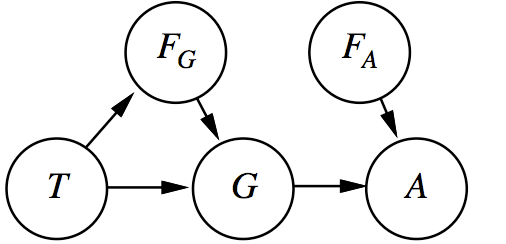
\includegraphics[width=\textwidth]{./images/nuclearpowerstationbayesiannet.png}
		\end{answer}
		\item Suppose there are just two possible actual and measured temperatures, normal and high, and the probability that the gauge gives the correct temperature is $x$ when it is working, but $y$ when it is faulty. Give the conditional probability table associated with node $G$.
		\marks{5}
		\begin{answer}
			Note the semantics of $F_G$ , which is true when the gauge is faulty, i.e., not working.
			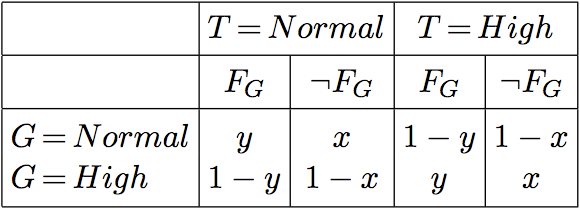
\includegraphics[width=\textwidth]{./images/cpt_node_g_q142.png}
		\end{answer}
		\end{enumerate}
		%bayesian learning
		\item Consider the following time keeping patterns of the lecturers in your college:
		\begin{itemize}
			\item 25\% of lecturers start 75\% of their lectures on time and 25\% late.
			\item 50\% of lecturers start 50\% of their lectures on time and 50\% late.
			\item 25\% of lecturers start 25\% of their lectures on time and 75\% late.
		\end{itemize}
		\begin{enumerate}
		\item Given that both the $1^{st}$ and $2^{nd}$ Artificial Intelligence lectures of the year started on time, compute the posterior probability that your Artificial Intelligence lecturer follows each of the three time keeping patterns.
		\marks{10}
		\begin{answer}
			To begin we will define some notation. Let: 
			\begin{itemize}
				\item $h_1$ denote the hypothesis that your AI lecturer starts 75\% of their lectures on time $P(h_1)=0.25$.
				\item $h_2$ denote the hypothesis that your AI lecturer starts 50\% of their lectures on time $P(h_2)=0.50$.
			   	\item $h_3$ denote the hypothesis that your AI lecturer starts 25\% of their lectures on time $P(h_3)=0.25$.
			\end{itemize}
			Also, if we use the notation $ontime_x$ to represent the observation that a lecture x started on time, then the probability of any given AI lecture starting on time given a particular hypothesis $h$ is:
			\begin{itemize}
				\item $P(ontime_x|h_1)=0.75$ .
				\item $P(ontime_x|h_2)=0.50$ .
				\item $P(ontime_x|h_3)=0.25$ .
			\end{itemize}
			Then:
			\begin{itemize}
				\item By Bayes' rule, we can compute the posterior probability of a hypothesis given the data so far using: 
				\begin{center}
					$P(h_i|\textbf{d}) = \alpha P(\textbf{d}|h_i) P(h_i)$
				\end{center}
				\item And, the likelihood of the data given a hypothesis is calculated using: 
				\begin{center}
					$P(\textbf{d}|h_i) = \prod_j P(d_j|h_i)$
				\end{center}
			\end{itemize}
			So:
			\begin{itemize}
				\item $P(h_1|ontime_1,ontime_2)=\alpha (\prod_{j=1}^2 P(ontime_j|h_1))P(h_1)=\alpha 0.75^2 \times 0.25=\alpha 0.375=\frac{0.375}{1.0} = 0.375$.
				\item $P(h_2|ontime_1,ontime_2)=\alpha (\prod_{j=1}^2 P(ontime_j|h_2))P(h_1)=\alpha 0.50^2 \times 0.50=\alpha 0.500=\frac{0.500}{1.0} = 0.500$.
				\item $P(h_3|ontime_1,ontime_2)=\alpha (\prod_{j=1}^2 P(ontime_j|h_3))P(h_1)=\alpha 0.25^2 \times 0.25=\alpha 0.125=\frac{0.125}{1.0} = 0.125$.
			\end{itemize}
		\end{answer}
		\item Given that both the $1^{st}$ and $2^{nd}$ Artificial Intelligence lectures of the year started on time, what is the Bayesian Prediction that the $3^{rd}$ Artificial Intelligence lecture will start on time? 
			\marks{5}
		\begin{answer}
			Bayesian predictions use a likelihood-weighted sum over the hypotheses: 
			\begin{center}
				$P(X|\textbf{d})=\sum_i P(X|h_i)P(h_i|\textbf{d})$
			\end{center}
			In this instance we get:
			\begin{eqnarray*}
				P(ontime_{3}|\textbf{d})&=&\sum_i P(ontime_{3}|h_i)P(h_i|\textbf{d})\\
				&=& (0.75 * 0.375) + (0.5 * 0.5) + (0.25 *0.125)\\
				&=& 0.28125 + 0.25 + 0.03125\\
				&=& 0.5625			
			\end{eqnarray*}
		\end{answer}
		\end{enumerate}
	\end{enumerate} %end Q3

%
\newpage

%Q4
%Linear Regression Neural Nets, SVMs, Ensemble Learning
\question 
	\begin{enumerate}
		%Regression Learning
		\item The following model is commonly used for continuous prediction tasks:
		\begin{center}
			$y(x)=w_0 + w_1x_1 + \dots + w_Dx_D$
		\end{center}
		\begin{enumerate}
			\item Provide the name for this model and explain all terms.
			\marks{5}
			\begin{answer}
			Students should explain that this is a simple linear regression model which can be effectively used to make predictions. $x$ is a vector of feature values for a query instance and $w$ is a vector of feature weights. An diagram of a simple one dimensional linear function would help.
			\end{answer}
			\item Briefly describe a technique for finding optimal values for the terms $w_0, w_1, \dots , w_D$ in the model based on a historical training set.
			\marks{5}
			\begin{answer}
			Students should explain that given a training set the performance of a particular linear regression model can be measured using an appropriate evaluations function, e.g. the \emph{sum of squares error} as follows:
			\begin{center}
				$E(w)=\frac{1}{2}\sum_{n=1}^{N}(y(x_n)-t_n)^2$
			\end{center}
			where $t_n$ is the \emph{true} answer for training instance $x_n$ and $y(x_n)$ is the prediction made by the model for instance $x_n$. Optimal values for $w$ are found by minimising E(w).
			\end{answer}
			\end{enumerate}
		%Neural Nets	
		\item Figure \ref{fig:nn} shows a backprogation network that is currently processing the training vector $[1.0, 0.9, 0.9]$ which has an  associated target vector $[0.1, 0.9, 0.1]$. Given that the output from unit B is $0.6$ and from C is $0.8$, and assuming that the activation function used at all nodes in the network is the logistic function (i.e., $f(x) = \frac{1}{1 + \exp^{-x}}$): 
		\begin{enumerate}
			\item Calculate the actual output vector (to 3 decimal places).
			\marks{5}
			\begin{answer}
				Output of unit $i = f(\sum_{j=1}^{n}W_{j,i}\times activation_j)$\\
				First output unit input = -0.3 x 0.6 + 0.9 x 0.8 = 0.54 $\rightarrow$ f(0.54) = 0.632\\
				Second output unit input = -0.6 x 0.6 + -0.1 x 0.8 = -0.44 $\rightarrow$ f(-0.44) = 0.392\\
				Third output unit input = 0.4 x 0.6 + 1.2 x 0.8 = 1.2 $\rightarrow$ f(1.2)= 0.769\\
			\end{answer}
			\item Calculate the error for each output unit.
			\marks{5}
			\begin{answer}
				Error =  target - output\\
				First output unit = (0.1 - 0.632)  = - 0.532\\
				Second output unit = (0.9 - 0.392) = 0.508\\
				Third output unit = (0.1 - 0.769) = - 0.696\\
			\end{answer}
			\item Calculate the error for each hidden unit B and C.
			\marks{10}
			\begin{answer}
				Each hidden node $j$ is responsible for some fraction of the error $Err_i$ of each of the output units $i$ to which it connects. Thus the $Err_i$ values are divided according to the strengths of the connection between the hidden node and the output nodes and are propagated back to the hidden nodes. Where a hidden node feeds-forward into more than 1 output node the errors propagated back to it are summed: $Err_j = \sum_{i=1}^{n}W_{ji} \times Err_i$:
				$Err_{B} = (-0.3 \times -0.532) + (-0.6 \times 0.508) + (0.4 \times -0.696) = 0.1596 + -0.3048 + -0.2784 = -0.4236$\\
				$Err_{C} = (0.9 \times -0.532) + (-0.1 \times 0.508) + (1.2 \times -0.696) =  -0.4788 + -0.0508 + -0.8352  = -1.3648$\\
			\end{answer}		
		\end{enumerate}
	\end{enumerate}

\begin{figure}[htbp]
\begin{center}
\includegraphics[width=3.5in]{./images/nn_callan_q10_2.png}
\caption{Example Neural Net}
\label{fig:nn}
\end{center}
\end{figure}


\end{document}
